\chapter{Introduction}

\chapter{Fuzzy Variables}

\section{Input Variables}

There are four input variables used in this fuzzy system that describe relevant features of each player of the game. The variables \texttt{daysPerWeek} and \texttt{minutesPerDay} describe the players commitment to the game measured in time units. The variables \texttt{currentLevel} and \texttt{currentPoint} describe the players progress in the game. The linguistic labels for each variable, as well as their value range and membership functions are described and justified in the following subsections. 

\subsection{daysPerWeek}

The \texttt{daysPerWeek} variable describes the activeness of the user measured in days per week on a scale from 0 to 7 with three linguistic labels: 'occasionally', 'regularly' and 'fully'. The respective membership functions are trapezoidal, their parameters can be seen in table \ref{tab:daysPerWeek}:

\begin{table}[H]
\centering
\begin{tabular}{@{}lll@{}}
\toprule
\textbf{linguistic label}  & \textbf{trapezoidal function} \\ 
\midrule
occasionally  & $(0,0,2,3)$ \\
regularly & $(2,3,5,6)$ \\
fully & $(5,6,7,7)$ \\
\bottomrule
\end{tabular}
\caption{Linguistic labels for \texttt{daysPerWeek}}
\label{tab:daysPerWeek}
\end{table}

As we can see graphically in figure \ref{fig:daysPerWeek}, the membership functions are not balanced. The labels 'occasionally' and 'regularly' take up more of the possible values than 'fully'.

\begin{figure}[H]
\centering
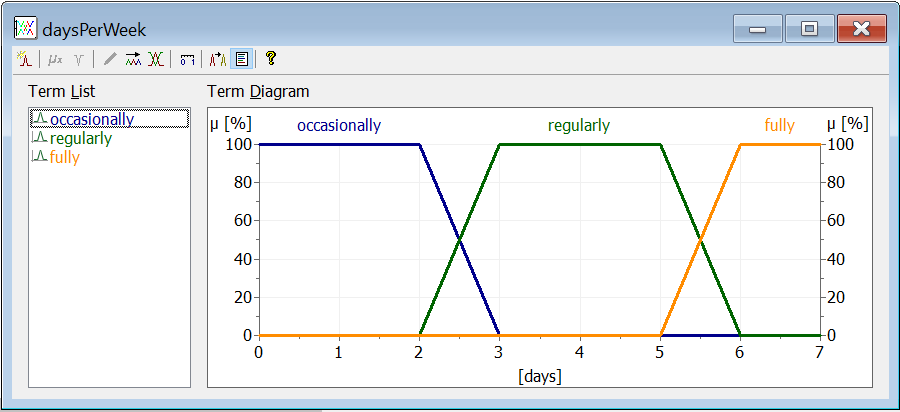
\includegraphics[width=\textwidth]{img/vDaysPerWeek}
\caption{Membership functions of \texttt{daysPerWeek} variable}
\label{fig:daysPerWeek} 
\end{figure}

\subsection{minutesPerDay}

The \texttt{minutesPerDay} variable describes the activeness of the user measured in minutes per day on a scale from 0 to 180 with four linguistic labels: 'negligible', 'short', 'right',  and 'large'. The respective membership functions are trapezoidal, their parameters can be seen in table \ref{tab:minutesPerDay}:

\begin{table}[H]
\centering
\begin{tabular}{@{}lll@{}}
\toprule
\textbf{linguistic label}  & \textbf{trapezoidal function} \\ 
\midrule
negligible  & $(0,0,5,15)$ \\
short & $(5,15,25,30)$ \\
right & $(25,30,60,90)$ \\
large & $(60,90,180,180)$ \\
\bottomrule
\end{tabular}
\caption{Linguistic labels for \texttt{minutesPerDay}}
\label{tab:minutesPerDay}
\end{table}

As we can see graphically in figure \ref{fig:minutesPerDay}, the membership functions are not balanced. The labels 'negligible' and 'short' have a relatively small value range, while 'large' alone covers more than half of the possible values.

\begin{figure}[H]
\centering
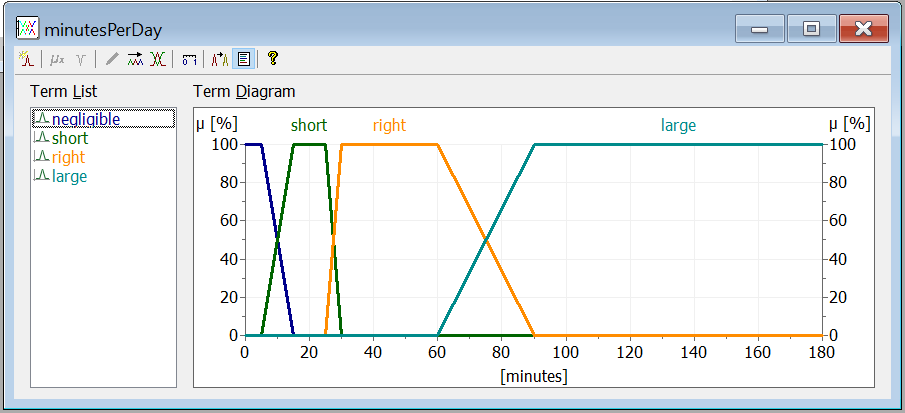
\includegraphics[width=\textwidth]{img/vMinutesPerDay}
\caption{Membership functions of \texttt{minutesPerDay} variable}
\label{fig:minutesPerDay} 
\end{figure}

\subsection{currentLevel}

The input varialbe \texttt{currentLevel} describes the progress of the user in the game measured with his current level. Its values range from 1 (start level) to 60 (maximum level). There are three linguistic labels to describe a player: 'beginner' for new players who do not have a lot of experience, 'intermediate' for players with some experience who still haven't proceeded to the late stage of the game, and 'advanced' for players who are close to finishing the game. The membership functions of these labels can be seen in table \ref{tab:currentLevel}.

\begin{table}[H]
\centering
\begin{tabular}{@{}lll@{}}
\toprule
\textbf{linguistic label}  & \textbf{trapezoidal function} \\ 
\midrule
beginner  & $(0,0,10,20)$ \\
intermediate & $(10,20,40,50)$ \\
advanced & $(40,50,60,60)$ \\
\bottomrule
\end{tabular}
\caption{Linguistic labels for \texttt{currentLevel}}
\label{tab:currentLevel}
\end{table}

The labels of \texttt{currentLevel} are unbalanced. The range of levels for which players are considered to be 'intermediate' is wider than for both 'beginner' and 'advanced'. This reflects the notion that players surmount the 'beginner' stadium rather quickly but then need a relatively long time to proceed towards being 'advanced'. This can be observed graphically in the plot of membership functions in figure \ref{fig:currentLevel}.

\begin{figure}[H]
\centering
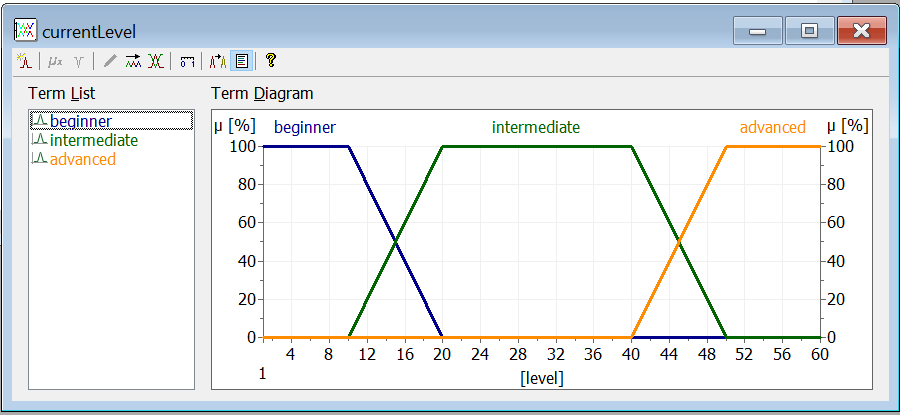
\includegraphics[width=\textwidth]{img/vCurrentLevel}
\caption{Membership functions of \texttt{currentLevel} variable}
\label{fig:currentLevel} 
\end{figure}

\subsection{currentPoints}

The variable \texttt{currentPoints} describes the amount of points of a player with the four linguistic labels 'few', 'some', 'average', and 'many'. A player can have between 0 and 1000 points and based on the current number of points and the membership functions of the labels, it gets assigned certain degrees of membership to the labels. The parameters of the trapezoidal membership functions are summarized in table \ref{tab:currentPoints}.

\begin{table}[H]
\centering
\begin{tabular}{@{}lll@{}}
\toprule
\textbf{linguistic label}  & \textbf{trapezoidal function} \\ 
\midrule
few  & $(0,0,100,150)$ \\
some & $(100,150,400,500)$ \\
average & $(400,500,700,800)$ \\
many & $(700,800,1000,1000)$ \\
\bottomrule
\end{tabular}
\caption{Linguistic labels for \texttt{currentPoints}}
\label{tab:currentPoints}
\end{table}

The unbalanced labels reflect the subjective judgement when saying 'few' or 'some': \textit{``a few points''} is a more narrow concept that \textit{``some points''}. This can be seen in the plotted membership functions in figure \ref{fig:currentPoints}. 

\begin{figure}[H]
\centering
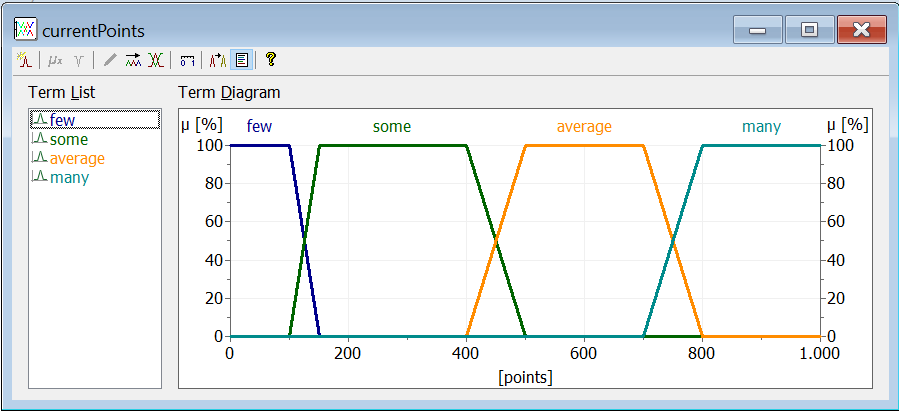
\includegraphics[width=\textwidth]{img/vCurrentPoints}
\caption{Membership functions of \texttt{currentPoints} variable}
\label{fig:currentPoints} 
\end{figure}

\section{Output Variables}

The system has two output variables: \texttt{addictionDegree} and \texttt{waitingMinutes}. The former describes the degree to which a player is addicted to the game. The latter defines how long a user needs to wait after loosing his lives in the game until he can start playing again. The more committed a player is to the game and the more advanced he is, the longer he should be asked to wait in order to increase the probabilities of them spending money on shortening the waiting time. Thus, the \texttt{addictionDegree} variable is both an output variable and an input variable to determine the best value for \texttt{waitingMinutes}. A more detailed overview of the connections between the variables and rule blocks is given in chapter \ref{cha:rb}.

\subsection{addictionDegree}

The output variable \texttt{addictionDegree} defines a players level of addiction to the game. The values range from 0 to 100 and are covered by three labels: 'lazy', 'normal' and 'eager'. The membership functions for these labels are trapezoidal and their parameters can be seen in table \ref{tab:addictionDegree}.

\begin{table}[H]
\centering
\begin{tabular}{@{}lll@{}}
\toprule
\textbf{linguistic label}  & \textbf{trapezoidal function} \\ 
\midrule
lazy  & $(0,0,15,25)$ \\
normal & $(15,25,75,85)$ \\
eager & $(75,85,100,100)$ \\
\bottomrule
\end{tabular}
\caption{Linguistic labels for \texttt{addictionDegree}}
\label{tab:addictionDegree}
\end{table}

The labels are unbalanced - players are considered to have a 'normal' addiction degree for a larger range of values than being considered 'lazy' or 'eager'. This corresponds to the subjective human understanding of addiction degree. The membership functions are plotted in figure \ref{fig:addictionDegree}.

\begin{figure}[H]
\centering
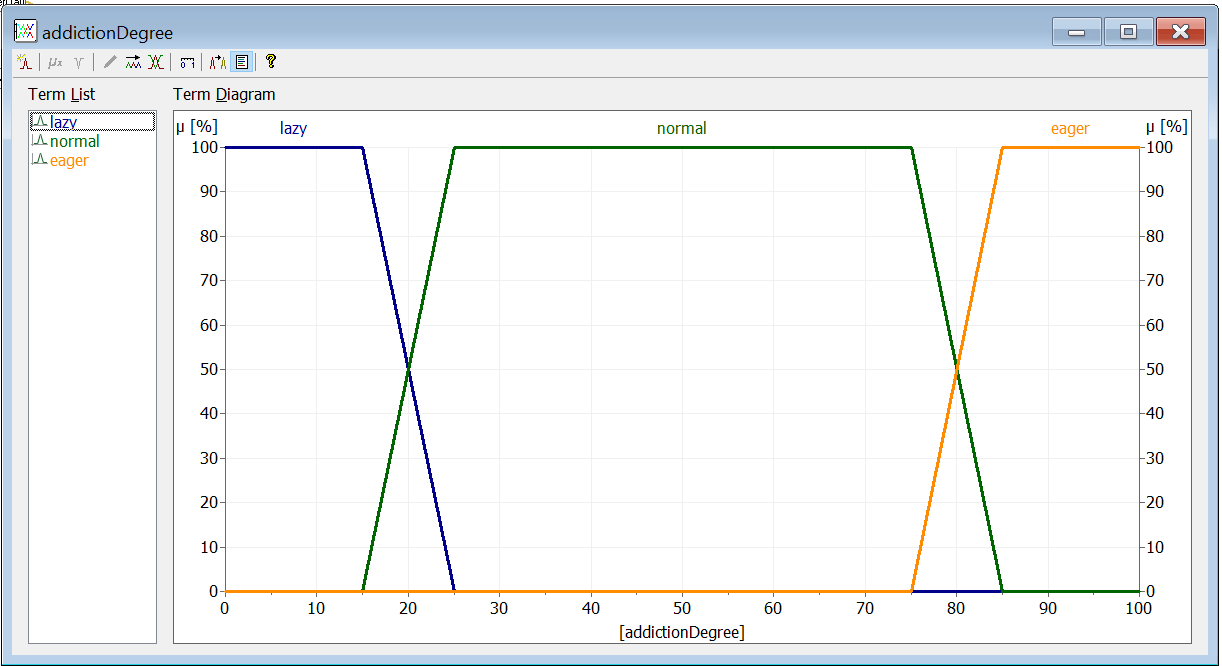
\includegraphics[width=\textwidth]{img/vAddictionDegree}
\caption{Membership functions of \texttt{addictionDegree} variable}
\label{fig:addictionDegree} 
\end{figure}

\subsection{waitingMinutes}

The variable \texttt{waitingMinutes} outputs how long a player needs to wait after loosing their in-game lives. If a player needs to wait too long it might lead to them abandoning the game. On the other hand, if the waiting time is too short to begin with, they will not spend money on making it shorter. The waiting time is always within a range between 0 and 120 minutes and is divided into five linguistic labels: 'veryShort', 'short', 'medium', 'long', and 'almostForever'. Their corresponding trapezoidal membership functions are depicted in table \ref{tab:waitingMinutes}.

\begin{table}[H]
\centering
\begin{tabular}{@{}lll@{}}
\toprule
\textbf{linguistic label}  & \textbf{trapezoidal function} \\ 
\midrule
veryShort  & $(0,0,5,10)$ \\
short & $(5,10,20,30)$ \\
medium & $(20,30,45,60)$ \\
long & $(45,60,90,105)$ \\
almostForever & $(90,105,120,120)$ \\
\bottomrule
\end{tabular}
\caption{Linguistic labels for \texttt{waitingMinutes}}
\label{tab:waitingMinutes}
\end{table}

The labels of \texttt{waitingMinutes} are distributed in an unbalanced way. The notion of 'veryShort', for example, lies on a much narrower value range than that of 'long'. This can be observed in the plotted membership functions of figure \ref{fig:waitingMinutes}.

\begin{figure}[H]
\centering
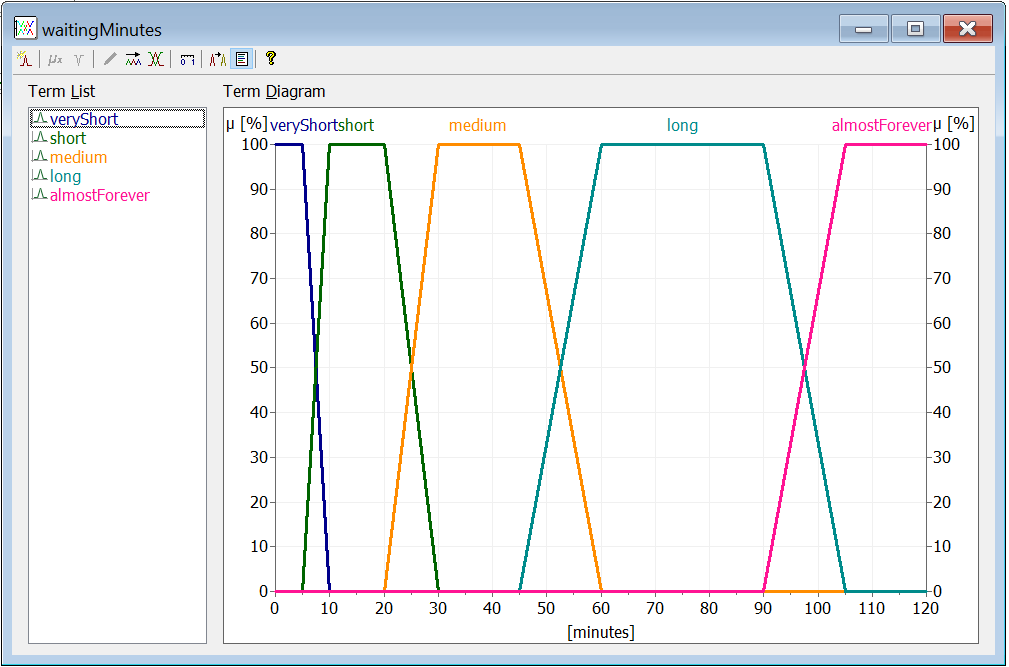
\includegraphics[width=\textwidth]{img/vWaitingMinutes}
\caption{Membership functions of \texttt{waitingMinutes} variable}
\label{fig:waitingMinutes} 
\end{figure}

\chapter{Rule Blocks}
\label{cha:rb}

The variables described in the previous section are connected by two rule blocks. The first rule block, described in section \ref{sec:rb1}, combines the input variables \texttt{minutesPerDay} and \texttt{daysPerWeek} to output a value of \texttt{addictionDegree}. The second rule block, described in section \ref{sec:rb2}, combines the output of the first rule block and the input variables \texttt{currentLevel} and \texttt{currentPoints} to output a value of \texttt{waitingMinutes}. The structure of the fuzzy system is shown in figure \ref{fig:all}.

\begin{figure}[H]
\centering
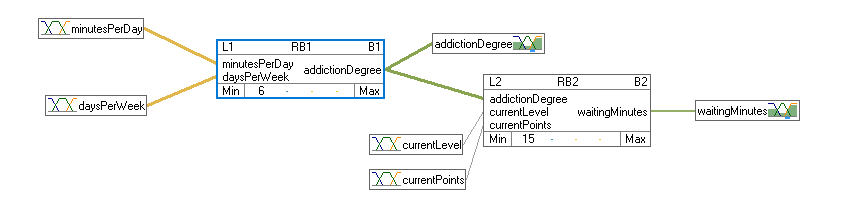
\includegraphics[width=\textwidth]{img/all}
\caption{Overview of variables and rule blocks}
\label{fig:all} 
\end{figure}

\section{Rules for addictionDegree}
\label{sec:rb1}

There are six fuzzy rules that combine the labels of \texttt{minutesPerDay} and \texttt{daysPerWeek} to deduce a label of \texttt{addictionDegree}. The first rule, \texttt{R1}, covers all cases in which the player plays only a 'negligible' amount of minutes per day: in these cases the \texttt{addictionDegree} is 'lazy'. The same deduction is done in \texttt{R2} for all players with the label \texttt{daysPerWeek.occasionally}. There are also conjunctive rules, such as \texttt{R4} in which a player is labelled as 'eager' if he has both the label \texttt{minutesPerDay.right} and \texttt{daysPerWeek.fully}. This rule block covers all possible combinations of the two input variables. Since the two input variables are probably highly correlated, in many cases one variable provides enough information about the player's addiction level. For example, if we know that a player plays only 'occasionally', the addiction degree will not be higher than 'lazy'. All rules can be seen in figure \ref{fig:rb1}.

\begin{figure}[H]
\centering
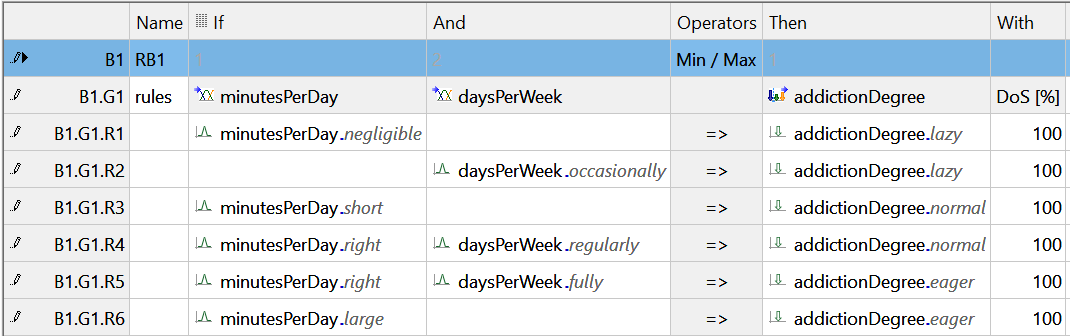
\includegraphics[width=\textwidth]{img/rb1}
\caption{Rule block for addictionDegree}
\label{fig:rb1} 
\end{figure}

\section{Rules for waitingMinutes}
\label{sec:rb2}

The second rule block is larger and more complex - it combines three input variables (one of them being the output of rule block 1 and the other ones being \texttt{currentLevel} and \texttt{currentPoints}) to the \texttt{waitingMinutes} output variable. Generally, the \texttt{waitingMinutes} increase with higher addictionDegree of the player, since a high addiction makes the player willing to wait longer or even motivates him to spend money on the game. A higher level also correlates with a longer wait time - the player has potentially invested many resources into the game and is incentivized to stay longer. Similarly, a high number of points increases the waiting time and thus motivates the player to spend these points. There are 15 different rules in the rule block, all covering at least a conjunction of 2 input variables. All possible cases are covered by the rules, with some cases slightly overlapping. The specific rules are depicted in figure \ref{fig:rb2}.

\begin{figure}[H]
\centering
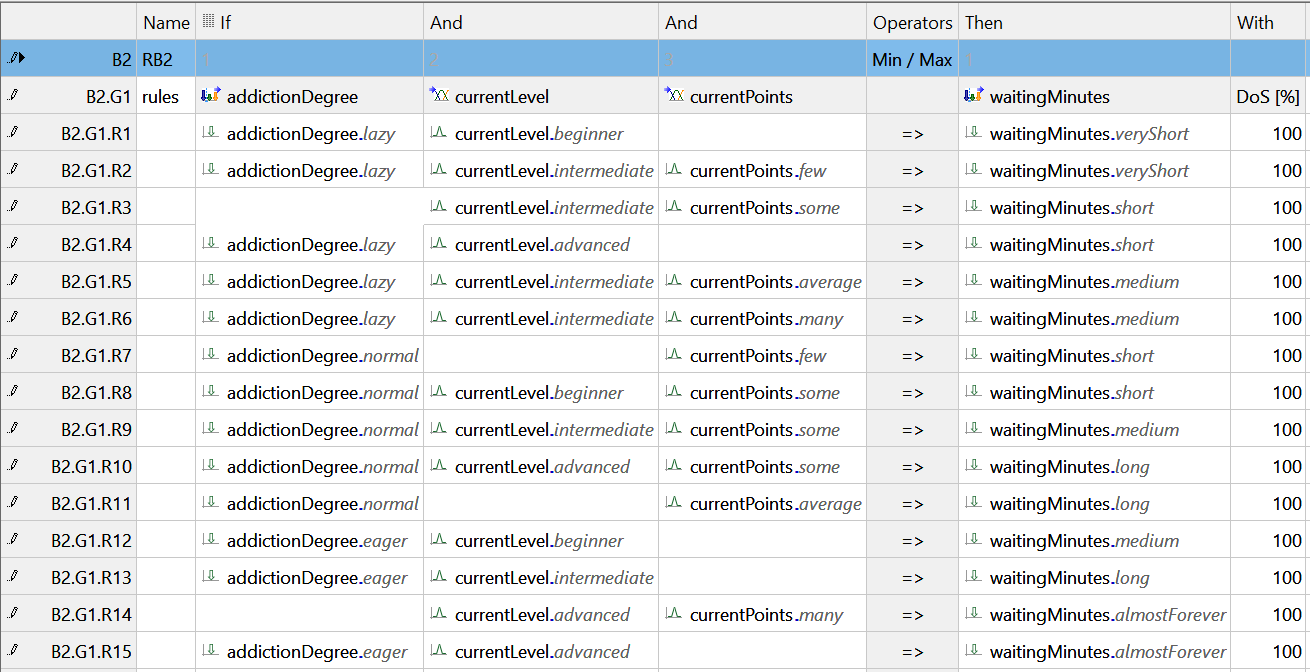
\includegraphics[width=\textwidth]{img/rb2}
\caption{Rule block for waitingMinutes}
\label{fig:rb2} 
\end{figure}

\chapter{Results}

\section{Manual calculation}

\subsection{User profile}

For the manual calculations based on the variables and rule blocks defined in the previous sections, a user profile was chosen that activates several labels and rules at the same time and is therefore interesting to observe. The chosen input variables are as summarized in table 

\begin{table}[H]
\centering
\begin{tabular}{@{}lll@{}}
\toprule
\textbf{variable}  & \textbf{input value} \\ 
\midrule
\texttt{minutesPerDay} & 83 \\
\texttt{daysPerWeek}  & 5.4 \\
\texttt{currentLevel} & 42 \\
\texttt{currentPoints} & 420 \\
\bottomrule
\end{tabular}
\caption{System input for manual calculations}
\label{tab:prof0}
\end{table}

\subsection{Fuzzyfication}
\label{sub:fuzzyfic}

The value $83$ for \texttt{minutesPerDay} lies between the labels 'right' $(25,30,60,90)$ and 'large' $(60,90,180,190)$.

\[ right: \frac{90-83}{90-60} \cdot 100\% = 23.\overline{3}\% \]
\[ large: \frac{83-60}{90-60} \cdot 100\% = 76.\overline{6}\% \]
\vspace{1em}

The value $5.4$ for \texttt{daysPerWeek} lies between the labels 'regularly' $(2,3,5,6)$ and 'fully' $(5,6,7,7)$.

\[ regularly: \frac{6-5.4}{6-5} \cdot 100\% = 60\% \]
\[ fully: \frac{5.4-5}{6-5} \cdot 100\% = 40\% \]
\vspace{1em}

The value $42$ for \texttt{currentLevel} lies between the labels 'intermediate' $(10,20,40,50)$ and 'advanced' $(40,50,60,60)$.

\[ intermediate: \frac{50-42}{50-40} \cdot 100\% = 80\% \]
\[ advanced: \frac{42-40}{50-40} \cdot 100\% = 20\% \]
\vspace{1em}

The value $420$ for \texttt{currentPoints} lies between the labels 'some' $(100,150,400,500)$ and 'average' $(400,500,700,800$).

\[ some: \frac{500-420}{500-400} \cdot 100\% = 80\% \]
\[ many: \frac{420-400}{500-400} \cdot 100\% = 20\% \]
\vspace{1em}

\subsection{Activation of addictionDegree}

The output variable \texttt{addictionDegree} depends on both \texttt{minutesPerDay} and \texttt{daysPerWeek}. From the previous section we know the activation of the labels for these two input variables: $23.\overline{3}\%$ for \texttt{minutesPerDay.right}, $76.\overline{6}\%$ for \texttt{large}, $60\%$ for \texttt{daysPerWeek.regularly}, and $40\%$ for \texttt{daysPerWeek.fully}. Looking at the rules in the relevant rule block (see section \ref{sec:rb1}) we can see that the following rules are activated:
\[ R4: right \wedge regularly \Rightarrow normal \]
\[ R5: right \wedge fully \Rightarrow eager \]
\[ R6: large \Rightarrow eager \]

Using the minimum operator for conjunctions, we obtain:

\[ R4: 23.\overline{3}\% \Rightarrow normal \]
\[ R5: 23.\overline{3}\% \Rightarrow eager \]
\[ R6: 76.\overline{6}\% \Rightarrow eager \]

Since we have several rules activating for the output label 'eager', we apply the maximum operator and obtain:

\[ 23.\overline{3}\% \Rightarrow normal \]
\[ 76.\overline{6}\% \Rightarrow eager \]

\subsection{Defuzzyfication of addictionDegree}

% --- normal:

To get the activated area of the 'normal' label we calculate the trapezoid of the label's membership function $(15,25,75,85)$ under the activation line $\mu = 23.\overline{3}$. The x-value of the intercept with the trapezoid and $\mu = 23.\overline{3}$ between $15$ and $25$ is:

\[ \frac{x_1-15}{25-15} \cdot 100\% = 23.\overline{3} \Leftrightarrow x_1 = 2.\overline{3} + 15 \Leftrightarrow x_1 = 17.\overline{3} \]

Equivalently, the intercept of the 'normal' trapezoid and $\mu = 23.\overline{3}$ between $75$ and $85$ is:

\[ \frac{85-x_2}{85-75} \cdot 100\% = 23.\overline{3} \Leftrightarrow x_2 = 85 - 2.\overline{3} \Leftrightarrow x_2 = 82.\overline{6} \]

Thus, the corner points of the resulting activated trapezoid are: 
\[A_{normal} = \{(15,0),(17.\overline{3},23.\overline{3}),(82.\overline{6},23.\overline{3}),(85,0) \}\]


% --- eager:

To get the activated area of the 'eager' label we calculate the trapezoid of the label's membership function $(75,85,100,100)$ under the activation line $\mu = 76.\overline{6}$. The x-value of the intercept with the trapezoid and $\mu = 76.\overline{6}$ between $75$ and $80$ is:

\[ \frac{x_1-75}{85-75} \cdot 100\% = 76.\overline{6} \Leftrightarrow x_1 =  82.\overline{6} \]

The resulting corner points of the activated trapezoid are:

\[A_{eager} = \{(75,0), (82.\overline{6},76.\overline{6}), (100,76.\overline{6}), (100,0) \}\]

We now have to take the maximum of the activated areas $A_{normal}$ and $A_{eager}$ for each $x$-value. $A_{normal}$ is obviously larger than $A_{eager}$ for $ x < 75 $. Thus, we have to find the intercept between  $A_{normal}$ and $A_{eager}$ in the range $ x \in [75, 82.\overline{6}]$ to determine the point $x^*$ at which $A_{eager}$ has higher $\mu$ values than $A_{normal}$ for $x > x^*$. We intercept the lines $\mu = 23.\overline{3}$ (coming from $A_{normal}$) and the line between $(75,0)$ and  $(82.\overline{6},76.\overline{6})$:

\[ \frac{x^*-75}{82.\overline{6}-75} \cdot 76.\overline{6}\% = 23.\overline{3} \Leftrightarrow x^* = 77.\overline{3} \]

With this information we know all corner points of the activated area for the \texttt{addictionDegree} variable:

\[ A_{addictionDegree} = \{ (15,0),(17.\overline{3},23.\overline{3}), (77.\overline{3},23.\overline{3}), (82.\overline{6},76.\overline{6}), (100,76.\overline{6}), (100,0)  \}\]

For defuzzyfication we use the \textit{Center of Area} (CoA) approach and try to find an $\overline{x}$ for which the activated area is the same on both sides.

To do this we first calculate the total area. We split up the shape into triangles and rectangles to calculate the area geometrically:

\[ A_{x \in [15,17.\overline{3}]} = \frac{1}{2} \cdot (17.\overline{3} - 15) \cdot (23.\overline{3} - 0 ) = 27.\overline{2} \]
\[ A_{x \in [17.\overline{3},77.\overline{3}]} = (77.\overline{3} - 17.\overline{3}) \cdot  (23.\overline{3} - 0 ) = 1400 \]
\[ A_{x \in [77.\overline{3},82.\overline{6}]} = (82.\overline{6} - 77.\overline{3}) \cdot ((23.\overline{3} - 0) + \frac{1}{2} \cdot (76.\overline{6} - (23.\overline{3})) = 266.\overline{6} \]
\[ A_{x \in [82.\overline{6},100]} = (100-82.\overline{6}) \cdot (76.\overline{6}-0) = 1328.\overline{8} \]

Summing up, we get to a total area of:

\[ A_{x \in [15,100]} = A_{x \in [15,17.\overline{3}]} + A_{x \in [17.\overline{3},77.\overline{3}]} + A_{x \in [77.\overline{3},82.\overline{6}]} + A_{x \in [82.\overline{6},100]} = 3022.\overline{6} \]

Thus, we are looking for $\overline{x}$ with 
\[ A_{x \in [15,\overline{x}]} = 3022.\overline{6} \cdot \frac{1}{2} = 1511.\overline{3} \]

We know that $A_{x \in [15,17.\overline{3}]} + A_{x \in [17.\overline{3},77.\overline{3}]} = 1427.\overline{2} $. Hence, we can reformulate the problem to find:

\[ A_{x \in [77.\overline{3},\overline{x}]} = 1511.\overline{3} - 1427.\overline{2} = 84.\overline{1} \]

Since $ A_{x \in [77.\overline{3},82.\overline{6}]} = 266.\overline{6} $ and $266.\overline{6} > 84.\overline{1}$ , we can search for a solution in the interval $[77.\overline{3},82.\overline{6}]$. The linear function that describes the top border of the area's segment between $[77.\overline{3},82.\overline{6}]$ can be described for $z = x -77.\overline{3}, x \in [77.\overline{3},82.\overline{6}] $ as

\[ f(z) = 23.\overline{3} + \frac{76.\overline{6} -23.\overline{3} }{82.\overline{6}-77.\overline{3}} \cdot z = 23.\overline{3} + 10z\]

We want to find $\overline{z}$ for which the integral of $f$ from 0 to $\overline{z}$ equals $84.\overline{1}$:

\[ \int_0^{\overline{z}} f(z) = 84.\overline{1} \Leftrightarrow [23.\overline{3}z + 5z^2]_0^{\overline{z}} = 84.\overline{1} \]

\[ \Rightarrow [23.\overline{3}\overline{z} + 5\overline{z}^2] - [0] = 84.\overline{1}\]

\[ \Rightarrow - 84.\overline{1} + 23.\overline{3}\overline{z} + 5\overline{z}^2  = 0\]

\[ \Rightarrow z_1 = 2.385, z_2 = -7.05 \]

Since $z$ can't be negative, we know that $\overline{z} = 2.385 $ and thus $\overline{x} = 2.385 + 77.\overline{3} $. We found the Center of Areas to be at an addiction degree of $79.7183$.

\subsection{Activation of waitingMinutes}

The output variable \texttt{waitingMinutes} depends on the two input variables \texttt{currentLevel} and \texttt{currentPoints}, as well as the output of \texttt{addictionDegree}. From section \ref{sub:fuzzyfic} we know the membership degrees of the labels for the two input variables. In the previous section we obtained the defuzzyfied value of the \texttt{addictionDegree} as $79.7183$. To make the following manual calculations a bit shorter while only slightly changing the final results, we round the \texttt{addictionDegree} up to $80.0$. This gives us an activation of \texttt{addictionDegree.normal} and \texttt{addictionDegree.eager} of exactly $50\%$ each. The activated rules of the rule block (see section \ref{sec:rb2}) are:

\[ R9: normal \wedge intermediate \wedge some \Rightarrow medium \]
\[ R10: normal \wedge advanced  \wedge some \Rightarrow long \]
\[ R13: eager \wedge intermediate \Rightarrow long \]
\[ R14: advanced \wedge many \Rightarrow almostForever \]
\[ R15: eager \wedge advanced \Rightarrow almostForever \]

Using the minimum operator for conjunctions, we obtain:

\[ R9: 20\% \Rightarrow medium \]
\[ R10: 20\% \Rightarrow long \]
\[ R13: 50\% \Rightarrow long \]
\[ R14: 20\% \Rightarrow almostForever \]
\[ R15: 20\% \Rightarrow almostForever \]

Since we have several rules activating for the output labels 'long' and 'almostForever', we apply the maximum operator and obtain:

\[ 20\% \Rightarrow medium \]
\[ 50\% \Rightarrow long \]
\[ 20\% \Rightarrow almostForever \]

\subsection{Defuzzyfication of waitingMinutes}

% --- medium:

To get the activated area of the 'medium' label we calculate the trapezoid of the label's membership function $(20,30,45,60)$ under the activation line $\mu = 20$. The x-value of the intercept with the trapezoid and $\mu = 20$ between $20$ and $30$ is:

\[ \frac{x_1-20}{30-20} \cdot 100\% = 20 \Leftrightarrow x_1 = 22 \]

Equivalently, the intercept of the 'medium' trapezoid and $\mu = 20$ between $45$ and $60$ is:

\[ \frac{60-x_2}{60-45} \cdot 100\% = 20 \Leftrightarrow x_2 = 57 \]

Thus, the corner points of the resulting activated trapezoid are: 
\[A_{medium} = \{ (20,0), (22,20), (57,20), (60,0) \}\]

% --- long:

To get the activated area of the 'long' label we calculate the trapezoid of the label's membership function $(45,60,90,105)$ under the activation line $\mu = 50$. The x-value of the intercept with the trapezoid and $\mu = 50$ between $45$ and $60$ is:

\[ \frac{x_1-45}{60-45} \cdot 100\% = 50 \Leftrightarrow x_1 = 52.5 \]

Equivalently, the intercept of the 'long' trapezoid and $\mu = 50$ between $90$ and $105$ is:

\[ \frac{105-x_2}{105-90} \cdot 100\% = 50 \Leftrightarrow x_2 = 97.5 \]

Thus, the corner points of the resulting activated trapezoid are: 
\[A_{long} = \{ (45,0), (52.5,50), (97.5,50), (105,0) \}\]


% --- almostForever:

To get the activated area of the 'almostForever' label we calculate the trapezoid of the label's membership function $(90,105,120,120)$ under the activation line $\mu = 20$. The x-value of the intercept with the trapezoid and $\mu = 20$ between $90$ and $105$ is:

\[ \frac{x_1-90}{105-90} \cdot 100\% = 20 \Leftrightarrow x_1 = 93 \]

Thus, the corner points of the resulting activated trapezoid are: 
\[A_{almostForever} = \{ (90,0),(93,20),(120,20),(120,0) \}\]


% --- total area:
We now have to take the maximum of the activated areas $A_{medium}$, $A_{long}$, and $A_{almostForever}$ for each $x$-value. $A_{medium}$ is  larger than $A_{long}$ for $ x < 45 $. Thus, we have to find the intercept between  $A_{medium}$ and $A_{long}$ in the range $ x \in [45,52.5]$ to determine the point $x^*$ at which $A_{long}$ has higher $\mu$ values than $A_{medium}$ for $x > x^*$. We intercept the lines $\mu = 20$ (coming from $A_{medium}$) and the line between $(45,0)$ and  $(52.5,50)$:

\[ \frac{x_1^*-45}{52.5-45} \cdot 50\% = 20 \Leftrightarrow x_1^* = 48 \]

$A_{almostForever}$ is  larger than $A_{long}$ for $ x > 105 $. Thus, we have to find the intercept between  $A_{almostForever}$ and $A_{long}$ in the range $ x \in [97.5,105]$ to determine the point $x^*$ at which $A_{long}$ has higher $\mu$ values than $A_{almostForever}$ for $x < x^*$. We intercept the lines $\mu = 20$ (coming from $A_{almostForever}$) and the line between $(97.5,50)$ and  $(105,0)$:

\[ \frac{105-x_2^*}{105-97.5} \cdot 50\% = 20 \Leftrightarrow x_2^* = 102 \]


With this information we know all corner points of the activated area for the \texttt{waitingMinutes} variable:

\[ A_{waitingMinutes} = \{ (20,0),(22,20),(48,20),(52.5,50),(97.5,50),(102,20),(120,20),(120,0)  \}\]

For defuzzyfication we use the \textit{Center of Area} (CoA) approach and try to find an $\overline{x}$ for which the activated area is the same on both sides.

To do this we first calculate the total area. We split up the shape into triangles and rectangles to calculate the area geometrically:

\[ A_{x \in [20,22]} = \frac{1}{2} \cdot (22-20) \cdot (20-0) = 20 \]
\[ A_{x \in [22,48]} = (48-22) \cdot (20-0) = 520 \]
\[ A_{x \in [48,52.5]} = (52.5-48) \cdot ((20-0) + \frac{1}{2}\cdot(50-20) ) = 157.5 \]
\[ A_{x \in [52.5,97.5]} = (97.5-52.5) \cdot (50-0) = 2250 \]
\[ A_{x \in [97.5,102]} = (102-97.5) \cdot ((20-0) + \frac{1}{2}\cdot(50-20) ) = 157.5 \]
\[ A_{x \in [102,120]} = (120-102) \cdot (20-0) = 360 \]

Summing up all areas we get:

\[ A_{x \in [20,120]} = 3465 \]

Thus, we are looking for $\overline{x}$ with 
\[ A_{x \in [20,120]} = 3465 \cdot \frac{1}{2} = 1732.5 \]

We know that $A_{x \in [20,52.5]}  = 697.5 $. Hence, we can reformulate the problem to find:

\[ A_{x \in [52.5,\overline{x}]} = 1732.5 - 697.5 = 1035 \]

Since the area $A_{x \in [52.5,97.5]}$ is a rectangle, we can obtain $\overline{x}$ with the equation 

\[ \overline{x} = 52.5 + \frac{1035}{2250} * (97.5-52.5) = 73.2 \]

Thus, the defuzzyfied value for \texttt{waitingMinutes} is $73.2$.

\section{Automatic calculation}

For the automatically calculated results, we define three user profiles with different, interesting features that lead to the activation of multiple rules at the same time. The user profiles are described in section \ref{sub:users} and the results of the fuzzy system are presented in section \ref{sub:autoRes}.

\subsection{User profiles}
\label{sub:users}

We define three user profiles reflecting different types of users: the 'enthusiastic beginner' (profile 1), the 'motivated veteran' (profile 2), and the 'skeptical beginner' (profile 3).

The 'enthusiastic beginner' has shortly started the game but is already spending a lot of time on it. His input variables can be seen in table \ref{tab:prof1}.

\begin{table}[H]
\centering
\begin{tabular}{@{}lll@{}}
\toprule
\textbf{variable}  & \textbf{input value} \\ 
\midrule
\texttt{minutesPerDay} & 80 \\
\texttt{daysPerWeek}  & 5.5 \\
\texttt{currentLevel} & 5 \\
\texttt{currentPoints} & 120 \\
\bottomrule
\end{tabular}
\caption{Input variables of profile 1: 'enthusiastic beginner'}
\label{tab:prof1}
\end{table} 

The 'motivated veteran' has played the game for a long time and while he is still an active player, his activity has gone down a bit recently. His input variables can be seen in table \ref{tab:prof2}

\begin{table}[H]
\centering
\begin{tabular}{@{}lll@{}}
\toprule
\textbf{variable}  & \textbf{input value} \\ 
\midrule
\texttt{minutesPerDay} & 28 \\
\texttt{daysPerWeek}  & 4 \\
\texttt{currentLevel} & 55 \\
\texttt{currentPoints} & 740 \\
\bottomrule
\end{tabular}
\caption{Input variables of profile 2: 'motivated veteran'}
\label{tab:prof2}
\end{table}

The 'skeptical beginner' is also fairly new to the game and is not yet convinced to spend a lot of time on playing it. His input variables can be seen in table \ref{tab:prof3}}

\begin{table}[H]
\centering
\begin{tabular}{@{}lll@{}}
\toprule
\textbf{variable}  & \textbf{input value} \\ 
\midrule
\texttt{minutesPerDay} & 12 \\
\texttt{daysPerWeek}  & 2.2 \\
\texttt{currentLevel} & 5 \\
\texttt{currentPoints} & 50 \\
\bottomrule
\end{tabular}
\caption{Input variables of profile 3: 'skeptical beginner'}
\label{tab:prof3}
\end{table}

\subsection{Results for output variables}
\label{sub:autoRes}